% Chapter 11

\chapter{Continuous cross over: pairings and pair wave functions} % Main chapter title

\label{Chapter11} % For referencing the chapter elsewhere, use \ref{Chapter9} 

\lhead{Part III. \emph{Two wires}}
\chead{Chapter 11. \emph{Pairings \& pair wave functions}} % This is for the header on each page - perhaps a shortened title
%----------------------------------------------------------------------------------------
In this chapter we investigate the functional behaviour of the pairings and pair wave functions as a function of the interwire distance, $d$, in the case of the energetically favourable continuous cross over. This is done in section \ref{sec.2wirespairingspairwavefunction}. Further, in section \ref{sec.2wirespairingstemperature} we investigate the temperature dependence of the pairings. 

\section{Functional behaviour} \label{sec.2wirespairingspairwavefunction}
In this section we numerically calculate the functional behaviour of the pairings and the pair wave functions for the continuous cross over. The analysis is performed in the same manner as in section \ref{sec.2wiresCrossover_energy}. 

For the sake of clarity we again write up the gap equations in the case $\Delta^{22}_k = - \Delta^{11}_k$ real and $\Delta^{12}_k$ purely imaginary, which we found to support the continuous cross over:
\begin{align}
\Delta^{11}_k &= -\frac{1}{\mathcal{L}}\sum_{k'} W_{\text{ind}}^{11}(k, k')\frac{\Delta^{11}_{k'}}{2E_{F,k'}}\tanh\left(\frac{\beta E_{F,k'}}{2}\right), \nonumber \\
\Delta^{12}_k &= -\frac{1}{\mathcal{L}}\sum_{k'} W_{\text{ind}}^{12}(k, k')\frac{\Delta^{12}_{k'}}{2E_{F,k'}}\tanh\left(\frac{\beta E_{F,k'}}{2}\right), \nonumber
\end{align} 
with $E_{F,k} = \sqrt{\varepsilon^2_k + (\Delta^{11}_k)^2 + |\Delta^{12}_k|^2}$. We numerically find self-consistent solutions to the above gap equations along with the number equation \eqref{eq.2wiresnumberequation}. This is summarized in figure \ref{fig.pairingkdependT0dvaried}. It explicitly shows, that the interwire pairing is even in $k$ and hence is a $s$-wave type pairing. We see, that it has its maximum value at $k = 0$ as one might expect from the interwire induced interaction. Further, it shows no oscillatory behaviour, it simply decays exponentially for large values of $k$. The intrawire pairing is seen to have the same functional form as for the single wire, hence a $p$-wave type pairing. The overall behaviour of the pairings are seen to be independent of $d$. The interwire pairing is simply enhanced as $d$ decreases, vice versa for the intrawire pairing.  

\begin{figure} 
\begin{center}  
% GNUPLOT: LaTeX picture with Postscript
\begingroup
  \makeatletter
  \providecommand\color[2][]{%
    \GenericError{(gnuplot) \space\space\space\@spaces}{%
      Package color not loaded in conjunction with
      terminal option `colourtext'%
    }{See the gnuplot documentation for explanation.%
    }{Either use 'blacktext' in gnuplot or load the package
      color.sty in LaTeX.}%
    \renewcommand\color[2][]{}%
  }%
  \providecommand\includegraphics[2][]{%
    \GenericError{(gnuplot) \space\space\space\@spaces}{%
      Package graphicx or graphics not loaded%
    }{See the gnuplot documentation for explanation.%
    }{The gnuplot epslatex terminal needs graphicx.sty or graphics.sty.}%
    \renewcommand\includegraphics[2][]{}%
  }%
  \providecommand\rotatebox[2]{#2}%
  \@ifundefined{ifGPcolor}{%
    \newif\ifGPcolor
    \GPcolorfalse
  }{}%
  \@ifundefined{ifGPblacktext}{%
    \newif\ifGPblacktext
    \GPblacktexttrue
  }{}%
  % define a \g@addto@macro without @ in the name:
  \let\gplgaddtomacro\g@addto@macro
  % define empty templates for all commands taking text:
  \gdef\gplbacktext{}%
  \gdef\gplfronttext{}%
  \makeatother
  \ifGPblacktext
    % no textcolor at all
    \def\colorrgb#1{}%
    \def\colorgray#1{}%
  \else
    % gray or color?
    \ifGPcolor
      \def\colorrgb#1{\color[rgb]{#1}}%
      \def\colorgray#1{\color[gray]{#1}}%
      \expandafter\def\csname LTw\endcsname{\color{white}}%
      \expandafter\def\csname LTb\endcsname{\color{black}}%
      \expandafter\def\csname LTa\endcsname{\color{black}}%
      \expandafter\def\csname LT0\endcsname{\color[rgb]{1,0,0}}%
      \expandafter\def\csname LT1\endcsname{\color[rgb]{0,1,0}}%
      \expandafter\def\csname LT2\endcsname{\color[rgb]{0,0,1}}%
      \expandafter\def\csname LT3\endcsname{\color[rgb]{1,0,1}}%
      \expandafter\def\csname LT4\endcsname{\color[rgb]{0,1,1}}%
      \expandafter\def\csname LT5\endcsname{\color[rgb]{1,1,0}}%
      \expandafter\def\csname LT6\endcsname{\color[rgb]{0,0,0}}%
      \expandafter\def\csname LT7\endcsname{\color[rgb]{1,0.3,0}}%
      \expandafter\def\csname LT8\endcsname{\color[rgb]{0.5,0.5,0.5}}%
    \else
      % gray
      \def\colorrgb#1{\color{black}}%
      \def\colorgray#1{\color[gray]{#1}}%
      \expandafter\def\csname LTw\endcsname{\color{white}}%
      \expandafter\def\csname LTb\endcsname{\color{black}}%
      \expandafter\def\csname LTa\endcsname{\color{black}}%
      \expandafter\def\csname LT0\endcsname{\color{black}}%
      \expandafter\def\csname LT1\endcsname{\color{black}}%
      \expandafter\def\csname LT2\endcsname{\color{black}}%
      \expandafter\def\csname LT3\endcsname{\color{black}}%
      \expandafter\def\csname LT4\endcsname{\color{black}}%
      \expandafter\def\csname LT5\endcsname{\color{black}}%
      \expandafter\def\csname LT6\endcsname{\color{black}}%
      \expandafter\def\csname LT7\endcsname{\color{black}}%
      \expandafter\def\csname LT8\endcsname{\color{black}}%
    \fi
  \fi
    \setlength{\unitlength}{0.0500bp}%
    \ifx\gptboxheight\undefined%
      \newlength{\gptboxheight}%
      \newlength{\gptboxwidth}%
      \newsavebox{\gptboxtext}%
    \fi%
    \setlength{\fboxrule}{0.5pt}%
    \setlength{\fboxsep}{1pt}%
\begin{picture}(7200.00,5040.00)%
    \gplgaddtomacro\gplbacktext{%
      \csname LTb\endcsname%
      \put(165,2771){\makebox(0,0)[r]{\strut{}$-3$}}%
      \put(165,3212){\makebox(0,0)[r]{\strut{}$-1.5$}}%
      \put(165,3653){\makebox(0,0)[r]{\strut{}$0$}}%
      \put(165,4094){\makebox(0,0)[r]{\strut{}$1.5$}}%
      \put(165,4535){\makebox(0,0)[r]{\strut{}$3$}}%
      \put(360,2488){\makebox(0,0){\strut{} }}%
      \put(1125,2488){\makebox(0,0){\strut{} }}%
      \put(1890,2488){\makebox(0,0){\strut{} }}%
      \put(2654,2488){\makebox(0,0){\strut{} }}%
      \put(3419,2488){\makebox(0,0){\strut{} }}%
    }%
    \gplgaddtomacro\gplfronttext{%
      \csname LTb\endcsname%
      \put(-605,3653){\rotatebox{-270}{\makebox(0,0){\strut{}$\Delta_k, \varepsilon_k$}}}%
      \put(833,4378){\makebox(0,0){\strut{}$\nu = 1$}}%
    }%
    \gplgaddtomacro\gplbacktext{%
      \csname LTb\endcsname%
      \put(3584,2771){\makebox(0,0)[r]{\strut{} }}%
      \put(3584,3212){\makebox(0,0)[r]{\strut{} }}%
      \put(3584,3653){\makebox(0,0)[r]{\strut{} }}%
      \put(3584,4094){\makebox(0,0)[r]{\strut{} }}%
      \put(3584,4535){\makebox(0,0)[r]{\strut{} }}%
      \put(3779,2488){\makebox(0,0){\strut{} }}%
      \put(4544,2488){\makebox(0,0){\strut{} }}%
      \put(5309,2488){\makebox(0,0){\strut{} }}%
      \put(6074,2488){\makebox(0,0){\strut{} }}%
      \put(6839,2488){\makebox(0,0){\strut{} }}%
    }%
    \gplgaddtomacro\gplfronttext{%
      \csname LTb\endcsname%
      \put(4253,4378){\makebox(0,0){\strut{}$\nu = 1$}}%
    }%
    \gplgaddtomacro\gplbacktext{%
      \csname LTb\endcsname%
      \put(165,756){\makebox(0,0)[r]{\strut{}$-3$}}%
      \put(165,1197){\makebox(0,0)[r]{\strut{}$-1.5$}}%
      \put(165,1638){\makebox(0,0)[r]{\strut{}$0$}}%
      \put(165,2078){\makebox(0,0)[r]{\strut{}$1.5$}}%
      \put(165,2519){\makebox(0,0)[r]{\strut{}$3$}}%
      \put(360,473){\makebox(0,0){\strut{}$-\pi$}}%
      \put(1125,473){\makebox(0,0){\strut{}$-\frac{\pi}{2}$}}%
      \put(1890,473){\makebox(0,0){\strut{}$0$}}%
      \put(2654,473){\makebox(0,0){\strut{}$\frac{\pi}{2}$}}%
      \put(3419,473){\makebox(0,0){\strut{}$\pi$}}%
    }%
    \gplgaddtomacro\gplfronttext{%
      \csname LTb\endcsname%
      \put(-605,1637){\rotatebox{-270}{\makebox(0,0){\strut{}$\Delta_k, \varepsilon_k$}}}%
      \put(1889,143){\makebox(0,0){\strut{}$kd$}}%
      \put(833,2362){\makebox(0,0){\strut{}$\nu = 0$}}%
    }%
    \gplgaddtomacro\gplbacktext{%
      \csname LTb\endcsname%
      \put(3584,756){\makebox(0,0)[r]{\strut{} }}%
      \put(3584,1197){\makebox(0,0)[r]{\strut{} }}%
      \put(3584,1638){\makebox(0,0)[r]{\strut{} }}%
      \put(3584,2078){\makebox(0,0)[r]{\strut{} }}%
      \put(3584,2519){\makebox(0,0)[r]{\strut{} }}%
      \put(3779,473){\makebox(0,0){\strut{}$-\pi$}}%
      \put(4544,473){\makebox(0,0){\strut{}$-\frac{\pi}{2}$}}%
      \put(5309,473){\makebox(0,0){\strut{}$0$}}%
      \put(6074,473){\makebox(0,0){\strut{}$\frac{\pi}{2}$}}%
      \put(6839,473){\makebox(0,0){\strut{}$\pi$}}%
    }%
    \gplgaddtomacro\gplfronttext{%
      \csname LTb\endcsname%
      \put(5309,143){\makebox(0,0){\strut{}$kd$}}%
      \put(4253,2362){\makebox(0,0){\strut{}$\nu = 2$}}%
    }%
    \gplbacktext
    \put(0,0){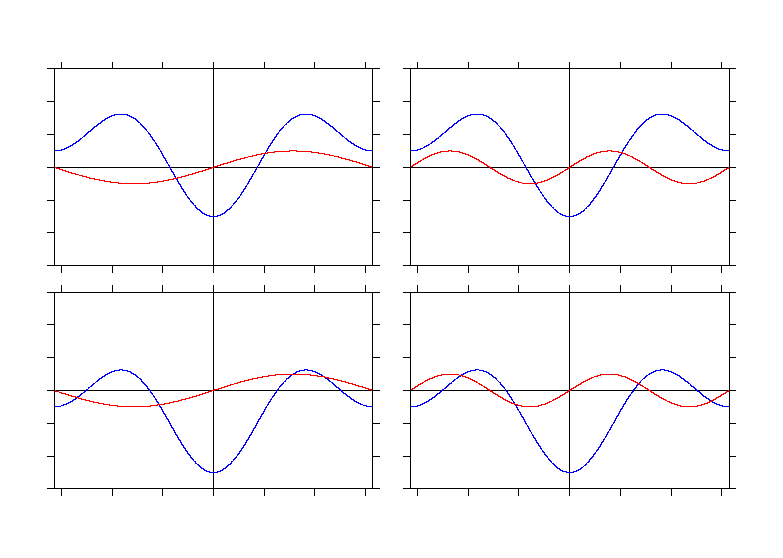
\includegraphics{Figures/Lattice.singlewire/dispersion/kdepend}}%
    \gplfronttext
  \end{picture}%
\endgroup
  
\caption{The pairings $\Delta^{11}_k$ (odd) and $\Delta^{12}_k$ (even) plotted as a function of $k$ for $\Delta^{12}_k$ imaginary. We see, that the functional behaviour is independent of $d$, and that there is a cross over between interwire and intrawire dominated pairing. The intrawire pairing is increased as $d$ increases. Vice versa for the interwire pairing. Parameters: $(n_Ba_B^3)^{1/3} = 0.01$, $(n_Ba_{BF}^3)^{1/3} = 0.11$, $l_t = 0$, $\frac{m_B}{m_F} = 7/40$, $\frac{n_F}{n_B^{1/3}} = 0.215$, $v_F/c_0 = 0.33$. }  
\label{fig.pairingkdependT0dvaried}  
\end{center}    
\end{figure}

To get a physically clearer picture of the effect of the pairings we calculate the pair wave functions in real space as well. Analogous to the calculation in subsection \ref{subsec.1wirepairwavefunction} we get the pair wave functions:
\begin{align}
\braket{\psi_{1,F}(x)\psi_{1,F}(0)} = - \braket{\psi_{2,F}(x)\psi_{2,F}(0)} &= \frac{i}{\mathcal{L}}\sum_k \sin(kx) \frac{\Delta^{11}_k}{2E_{F,k}}\tanh\left[\frac{ \beta E_{F,k} }{2}\right], \nonumber \\
\braket{\psi_{1,F}(x)\psi_{2,F}(0)} &= \frac{1}{\mathcal{L}}\sum_k \cos(kx) \frac{\Delta^{12}_k}{2E_{F,k}}\tanh\left[\frac{ \beta E_{F,k} }{2}\right].
\label{eq.2wirespairwavefunctionsDelta12imaginary}
\end{align} 
Here we should note, that if $E^\pm_{F,k} \neq E_{F,k}$ then the above pair wave functions will be altered. From this we can infer an overall functional behaviour. Firstly, we see that $\braket{\psi_{1,F}(x)\psi_{1,F}(0)}$ and $\braket{\psi_{1,F}(x)\psi_{2,F}(0)}$ are respectively odd and even in $x$. Further, since $\sin(kx)$ and $\cos(kx)$ oscillates more rapidly as a function of $k$ at higher values of $x$ we expect the pair wave functions to decay to 0. This is also physically reasonable.  

As noted in subsection \ref{subsec.1wirepairwavefunction}, the pair wave function is a measure of the spatial correlations between the fermions. Hence, a high value of $\left|\braket{\psi_{1,F}(x)\psi_{1,F}(0)}\right|$ means, that there is a tendency of two particles in the same wire to have the interparticle distance $x$. Similarly a high value $\left|\braket{\psi_{1,F}(x)\psi_{2,F}(0)}\right|$ means, that if a fermion in wire 2 is located at $x' = 0$, there is a tendency of a second fermion to be located at the position $x$ in wire 1.  

\begin{figure} 
\begin{center}  
\input{Figures/twowires/pairwavefunctions/xdepend11.tex}  
\caption{The \textit{intra}wire pairwave function $\braket{\psi_{1,F}(x)\psi_{1,F}(0)}$ as a function of $x$ for $\Delta^{12}_k$ imaginary. We see, that the functional behaviour is independent of $d$, the pair wave function is simply decreased as $d$ decreases. Parameters: $(n_Ba_B^3)^{1/3} = 0.01$, $(n_Ba_{BF}^3)^{1/3} = 0.11$, $l_t = 0$, $\frac{m_B}{m_F} = 7/40$, $\frac{n_F}{n_B^{1/3}} = 0.215$, $v_F/c_0 = 0.33$. }  
\label{fig.2wirespairwavefunction11}  
\end{center}    
\end{figure}

\begin{figure} 
\begin{center}  
\input{Figures/twowires/pairwavefunctions/xdepend12.tex}  
\caption{The \textit{inter}wire pairwave function $\braket{\psi_{1,F}(x)\psi_{2,F}(0)}$ as a function of $x$ for $\Delta^{12}_k$ imaginary. We see, that the functional behaviour is independent of $d$, the pair wave function is simply increased as $d$ decreases. Parameters: $(n_Ba_B^3)^{1/3} = 0.01$, $(n_Ba_{BF}^3)^{1/3} = 0.11$, $l_t = 0$, $\frac{m_B}{m_F} = 7/40$, $\frac{n_F}{n_B^{1/3}} = 0.215$, $v_F/c_0 = 0.33$. }  
\label{fig.2wirespairwavefunction12}  
\end{center}    
\end{figure}

By using the pairings found in the above analysis we can readily calculate the pair wave functions numerically. The result is shown in figures \ref{fig.2wirespairwavefunction11} and \ref{fig.2wirespairwavefunction12}. They have the following physical interpretation. The \textit{intra}wire pair wave function of figure \ref{fig.2wirespairwavefunction11} has the exact same structure as in the single wire case. There is a high tendency of the particles to be a distance $1/k_F$ apart internally in each wire. Further, the correlation is decreased when we decrease the interwire distance, $d$, since the intrawire pairing decreases. The \textit{inter}wire pair wave function of figure \ref{fig.2wirespairwavefunction12}, shows that there is a tendency of a fermion in wire 1 to be facing a fermion in wire 2. As for the single wire case we can come with the following intuitive picture of how the pairings tend to order the system. When the wires are well separated the intrawire pairing dominates the interwire one. This means, that the fermions tend to have an interparticle distance of $1 / k_F$ internally in each wire, but there is no correlation of the positions between the wires. This is illustrated to the left in figure \ref{fig.2wirespositioncorrelations}. For intermediate distances both pairings are present and the system is ordered both with respect to the intrawire and interwire correlations. This is the middle of figure \ref{fig.2wirespositioncorrelations}. Finally for small interwire distances, only the interwire pairing is present: the system only orders with respect to the interwire correlation. 

\begin{figure}
\center
\begin{tikzpicture}

%Only intrawire: 
\node at (2, 3) {Only intrawire};

%correlations:
\draw[-, thick, blue] (6 * 1/3 - 1/6, 0.04) -- (6 * 1/3 - 1/6 + 0.2238, 1.96);  
\draw (6 * 1/3 - 1/6 + 0.1119, 1.0) node[cross, rotate=-6.384836653, thick, red]{}; 
\draw[-, thick, red]  (5 * 1/3 - 1/6 + 0.2238, 2.08) to[out=90, in=90, distance = 0.2cm] (6 * 1/3 - 1/6 + 0.2238, 2.08);

\draw[-, thick] (0, 0) -- (4, 0);
\draw[*-] (1 * 1/3 - 1/6, 0.08); 
\draw[*-] (2 * 1/3 - 1/6, 0.08); 
\draw[*-] (3 * 1/3 - 1/6, 0.08); 
\draw[*-] (4 * 1/3 - 1/6, 0.08); 
\draw[*-] (5 * 1/3 - 1/6, 0.08); 
\draw[*-] (6 * 1/3 - 1/6, 0.08); 
\draw[*-] (7 * 1/3 - 1/6, 0.08); 
\draw[*-] (8 * 1/3 - 1/6, 0.08); 
\draw[*-] (9 * 1/3 - 1/6, 0.08); 
\draw[*-] (10 * 1/3 - 1/6, 0.08); 
\draw[*-] (11 * 1/3 - 1/6, 0.08);
\draw[*-] (12 * 1/3 - 1/6, 0.08); 

\draw[-, thick] (0, 2) -- (4, 2);
\draw[*-] (1 * 1/3 - 1/6 + 0.2238, 2.08); 
\draw[*-] (2 * 1/3 - 1/6 + 0.2238, 2.08); 
\draw[*-] (3 * 1/3 - 1/6 + 0.2238, 2.08); 
\draw[*-] (4 * 1/3 - 1/6 + 0.2238, 2.08); 
\draw[*-] (5 * 1/3 - 1/6 + 0.2238, 2.08); 
\draw[*-] (6 * 1/3 - 1/6 + 0.2238, 2.08); 
\draw[*-] (7 * 1/3 - 1/6 + 0.2238, 2.08); 
\draw[*-] (8 * 1/3 - 1/6 + 0.2238, 2.08); 
\draw[*-] (9 * 1/3 - 1/6 + 0.2238, 2.08); 
\draw[*-] (10 * 1/3 - 1/6 + 0.2238, 2.08); 
\draw[*-] (11 * 1/3 - 1/6 + 0.2238, 2.08);
\draw[*-] (12 * 1/3 - 1/6 + 0.2238 - 4, 2.08);

%%%%%%%%

%BOTH: 
\node at (7, 3) {Both};

%correlations:
\draw[-, thick, blue] (5 + 6 * 1/3 - 1/6, 0.08) -- (5 + 6 * 1/3 - 1/6, 1.58);  
\draw[-, thick, red]  (5 + 5 * 1/3 - 1/6, 1.58) to[out=90, in=90, distance = 0.2cm] (5 + 6 * 1/3 - 1/6, 1.58);

\draw[-, thick] (5, 0) -- (9, 0);
\draw[*-] (1 * 1/3 - 1/6 + 5, 0.08); 
\draw[*-] (2 * 1/3 - 1/6 + 5, 0.08); 
\draw[*-] (3 * 1/3 - 1/6 + 5, 0.08); 
\draw[*-] (4 * 1/3 - 1/6 + 5, 0.08); 
\draw[*-] (5 * 1/3 - 1/6 + 5, 0.08); 
\draw[*-] (6 * 1/3 - 1/6 + 5, 0.08); 
\draw[*-] (7 * 1/3 - 1/6 + 5, 0.08); 
\draw[*-] (8 * 1/3 - 1/6 + 5, 0.08); 
\draw[*-] (9 * 1/3 - 1/6 + 5, 0.08); 
\draw[*-] (10 * 1/3 - 1/6 + 5, 0.08); 
\draw[*-] (11 * 1/3 - 1/6 + 5, 0.08);
\draw[*-] (12 * 1/3 - 1/6 + 5, 0.08);

\draw[-, thick] (5, 1.5) -- (9, 1.5);
\draw[*-] (1 * 1/3 - 1/6 + 5, 1.58); 
\draw[*-] (2 * 1/3 - 1/6 + 5, 1.58); 
\draw[*-] (3 * 1/3 - 1/6 + 5, 1.58); 
\draw[*-] (4 * 1/3 - 1/6 + 5, 1.58); 
\draw[*-] (5 * 1/3 - 1/6 + 5, 1.58); 
\draw[*-] (6 * 1/3 - 1/6 + 5, 1.58); 
\draw[*-] (7 * 1/3 - 1/6 + 5, 1.58); 
\draw[*-] (8 * 1/3 - 1/6 + 5, 1.58); 
\draw[*-] (9 * 1/3 - 1/6 + 5, 1.58); 
\draw[*-] (10 * 1/3 - 1/6 + 5, 1.58); 
\draw[*-] (11 * 1/3 - 1/6 + 5, 1.58);
\draw[*-] (12 * 1/3 - 1/6 + 5, 1.58);

%%%%%%%%

%Only intrawire:
\node at (12, 3) {Only interwire};

%correlations:
\draw[-, thick, blue] (1.8932 + 10, 0.04) -- (1.8932 + 10, 0.96);  
\draw[-, thick, red]  (1.4066 + 10, 1.08) to[out=90, in=90] (1.8932 + 10, 1.08);
\draw (1.4066 + 10 + 0.2433, 1.215) node[cross, thick, blue]{}; 

\draw[-, thick] (10, 0) -- (14, 0);
\draw[*-] (0.7864 + 10, 0.08); 
\draw[*-] (0.9741 + 10, 0.08); 
\draw[*-] (1.0043 + 10, 0.08); 
\draw[*-] (1.3999 + 10, 0.08); 
\draw[*-] (1.4066 + 10, 0.08); 
\draw[*-] (1.8932 + 10, 0.08); 
\draw[*-] (2.1989 + 10, 0.08); 
\draw[*-] (2.3411 + 10, 0.08); 
\draw[*-] (2.4642 + 10, 0.08); 
\draw[*-] (3.2571 + 10, 0.08); 
\draw[*-] (3.3233 + 10, 0.08);
\draw[*-] (3.7171 + 10, 0.08);

\draw[-, thick] (10, 1) -- (14, 1);
\draw[*-] (0.7864 + 10, 1.08); 
\draw[*-] (0.9741 + 10, 1.08); 
\draw[*-] (1.0043 + 10, 1.08); 
\draw[*-] (1.3999 + 10, 1.08); 
\draw[*-] (1.4066 + 10, 1.08); 
\draw[*-] (1.8932 + 10, 1.08); 
\draw[*-] (2.1989 + 10, 1.08); 
\draw[*-] (2.3411 + 10, 1.08); 
\draw[*-] (2.4642 + 10, 1.08); 
\draw[*-] (3.2571 + 10, 1.08); 
\draw[*-] (3.3233 + 10, 1.08);
\draw[*-] (3.7171 + 10, 1.08);

\end{tikzpicture}
\caption{An intuitive picture of how the pairings tend to order the system. The fermions are depicted by black dots. The \textit{intra}wire and \textit{inter}wire correlation is depicted by red and blue lines respectively. Left: large interwire distance; only intrawire pairing present. The intrawire correlation ruins the interwire correlation, hence the red cross over the blue line. Middle: intermediate interwire distance; both pairings present. Both types of correlation are present. Right: small interwire distance; only interwire pairing present. The \textit{inter}wire correlation ruins the intrawire correlation, hence the blue cross over the red line.}
\label{fig.2wirespositioncorrelations}
\end{figure}


We can also use this to come with an intuitive explanation of the uptil now curious fact, that the numerical analysis shows, that the chemical potential is decreased by the presence of the \textit{intra}wire and increased by the presence of the \textit{inter}wire pairing. Specifically at $T = 0$, when only intrawire pairing is present $\mu < \epsilon_{F,0}$ whilst for only interwire pairing: $\mu > \epsilon_{F,0}$. The above analysis shows, that the intrawire pairing makes sure, that the fermions to a higher degree stay out of each others way. Therefore the energy to put in an additional fermion $\mu = \partial E/\partial N_F$ is lowered. Oppositely, the interwire pairing has a tendency to accumulate lumps of fermions, and so the energy required to put in an additional fermion $\mu = \partial E/\partial N_F$ is increased. 

\section{Temperature dependency of pairings} \label{sec.2wirespairingstemperature}
In this section we will investigate, how the pairings depend on temperature. The analysis is performed in complete analogy to the one in subsection \ref{subsec.momentum_and_temperature_pairing_singlewire}. 

For small and large distances, where one of the pairings is dominant, it is not difficult to imagine, what will happen. Here we expect, that the two pairings go to zero in a similar manner to single wire at two different critical temperatures. The dominant pairing for $T = 0$ will have the highest critical temperature. However, a couple questions arise. How does it affect the dominant pairing, that the suppressed pairing goes to zero? And is the interwire or intrawire pairing the more robust to a rise in temperature?

To answer these questions we investigate three cases, two where one pairing is strongly dominant, and one where the pairings are essentially equal for $T = 0$. The more interesting case is definitely the latter one, since this directly tests what pairing is the more robust. However, we might also gain some insight from the former. 

The result of the analysis for a dominant interwire pairing is shown in figure \ref{fig.maximalpairingsTdepend_2wires}. We see, that the overall expected behaviour is observed. We observe that the intrawire pairing has a small downward kink, where the interwire pairing vanishes. The same behaviour is seen when the interwire pairing is dominant. This has to implications. The first is, that the dominant pairing would be higher at low temperatures if the other pairing was not present: there is a trade off between the size of the individual pairings and the presence of a second pairing. The second is, that the presence of a second smaller pairing seem to stabilize the dominant one, since the kink is downwards for increasing temperatures. Further, above the critical temperature of the smaller pairing, the maximal intrawire pairing of the dominating pairing is well described by the following relation:
\begin{equation}
\max_k[\Delta^{\text{dom}}_k(T)] = \alpha \max_k[\Delta^{\text{dom}}_k(T = 0)] \sqrt{1 - \left(\frac{T}{T_c}\right)^3},
\label{eq.DeltaapproxaboveTC1}
\end{equation}
where $\text{dom}$ is short for dominating. This has the same form as the approximate form in equation \eqref{eq.maxpairingapprox} apart from the $\alpha$. The coefficient $\alpha$ is slightly bigger than $1$, but seems to depend slightly on the other parameters of the problem. For the present set of parameters we have $\alpha = 1.3$. 

\begin{figure} 
\begin{center}  
\input{Figures/twowires/Deltas4.5/Tdepend.tex}  
\caption{Blue solid line: $\max_k[|\Delta^{12}_k|]$ as a function of temperature. Blue dashed line: approximate form from the single wire analysis, equation \eqref{eq.maxpairingapprox}. Red solid line: $\max_k[|\Delta^{11}_k|]$ as a function of temperature. Red dashed line: Approximate form according to equation \eqref{eq.DeltaapproxaboveTC1} above the critical temperature of the interwire pairing. Notice, that there are two critical temperatures, and that the intrawire pairing shows a downward kink, where the interwire pairing goes to zero. Parameters: $k_Fd = 0.61$, $(n_Ba_B^3)^{1/3} = 0.01$, $(n_Ba_{BF}^3)^{1/3} = 0.11$, $l_t = 0$, $\frac{m_B}{m_F} = 7/40$, $\frac{n_F}{n_B^{1/3}} = 0.215$, $v_F/c_0 = 0.33$.}  
\label{fig.maximalpairingsTdepend_2wires}  
\end{center}    
\end{figure} 
